\chapter{Query translation}
Following the abstraction and conversion processes established for entities and mapping, query translation can be approached in a similar manner. By comparing query concepts across \acrshort{orm} frameworks, a unified abstraction can be derived. Once this abstraction is defined, the full translation process can be formulated, along with algorithms demonstrating its application. 


\section{Query abstraction}
The analyzed frameworks offer only two main query languages - \acrshort{sql} and \acrshort{linq}. RepoDB's lambda expressions can be considered a very limited subset of \acrshort{linq}, while \acrshort{hql}, used only by NHibernate, is syntactically similar to \acrshort{sql} sees minimal adoption and is not recommended\footnote{\url{https://www.red-gate.com/simple-talk/development/dotnet-development/some-nhibernate-best-practices/\#forget-about-hql}}. As discussed in \autoref{sec:core_translation}, \acrshort{linq} is typically translated into \acrshort{sql} before the database query is executed. Therefore, \acrshort{sql} can serve as a good foundation for abstraction. However, it is not used directly, as doing so would restrict potential future extensions. A simpler, yet less general approach---executing a \acrshort{linq} query, capturing the generated \acrshort{sql}, and reusing it with a raw \acrshort{sql} query method in another \acrshort{orm}-- is an approach not considered in this work.

While entity and mapping definitions follow a relatively limited set of formats and possibilities, parsing LINQ queries becomes a challenge of parsing arbitrary C\# code. Queries must be interpreted in the context of the framework and the surrounding method in which they appear. They are rarely standalone, often referencing method arguments or external variables. Each framework uses a distinct object to represent a database connection or session. This object is responsible for query initialization and typically exposes methods for executing raw \acrshort{sql}. For \acrshort{linq} queries, it provides access to the implementation of the \texttt{IQueryable}\footnote{\url{https://learn.microsoft.com/en-us/dotnet/csharp/linq/get-started/introduction-to-linq-queries\#the-data-source}} interface, parametrized with the source entity type and extended through chained \acrshort{linq} method calls.

\autoref{tab:query_comp}, based on the framework analysis in \autoref{chapter:ormcomparison}, summarizes the structure of supported queries. Rows represent key query components, and columns correspond to specific \acrshort{orm}s. As previously mentioned, only \acrshort{sql} and \acrshort{linq} queries are considered.

Queries primarily consist of the application code that defines the \textbf{query source}, \textbf{method}, and a \textbf{generic parameter} referencing entity. The query itself can be decomposed into parts: \textbf{projection}, \textbf{selection}, \textbf{joining}, \textbf{grouping}, \textbf{ordering} and \textbf{set operations}. 

Among the frameworks that support \acrshort{linq}, it is evident that they share common semantic operations, with occasional differences in method names (e.g., \texttt{LoadWith}, \texttt{Fetch}, \texttt{Include}). Translating a \acrshort{linq} query to another \acrshort{orm}'s \acrshort{linq} implementation could, in principle, be achieved by simple method renaming, without the need for an intermediate representation. However, this approach is not further explored in this work.

%\clearpage
\begin{landscape}
\begin{table}
\centering
\caption{Comparison of key query components across different frameworks.}
\label{tab:query_comp}
\scriptsize
\def\arraystretch{1.35}
\begin{tabular}{
>{\raggedright\arraybackslash}p{20.00mm}
>{\arraybackslash}p{30.00mm}
>{\arraybackslash}p{30.00mm}
>{\arraybackslash}p{30.00mm}
>{\arraybackslash}p{30.00mm}
>{\arraybackslash}p{30.00mm}
>{\arraybackslash}p{30.00mm}
}
\toprule
  &  \textbf{Dapper}\newline raw SQL &  \textbf{PetaPoco} \newline raw SQL/Sql.Builder &   \textbf{RepoDB} \newline lambda expressions &   \textbf{LINQ to DB} \newline LINQ & \textbf{NHibernate} \newline LINQ  &   \textbf{EF Core} \newline LINQ \\
\midrule

Query source  & SqlConnection & IDatabase & SqlConnection & DataConnection &  ISession & DbContext \\
\midrule

Raw SQL method  & \texttt{SqlConnection\newline.Query()} & \texttt{IDatabase\newline.Query()} & \texttt{SqlConnection\newline.ExecuteQuery()} & \texttt{DataConnection\newline.Query()} &  \texttt{ISession\newline.CreateSQLQuery()} & \texttt{DbContext\newline.SqlQueryRaw()} \\
\midrule

LINQ method & - & - & - & \texttt{DataConnection\newline.GetTable<>()} & \texttt{ISession\newline.Query<>()} & \texttt{DbContext\newline.DBSet<>()} \\
\midrule

Source table  & FROM & FROM or entity mapping & entity mapping  & entity mapping &  entity mapping & entity mapping \\
\midrule

Projection & SELECT $\ldots$ & \texttt{Sql.Builder} automatically from entity & \texttt{Field.From()}  & default entity, modified with \texttt{Select()} & default entity, modified with \texttt{Select()} & default entity, modified with \texttt{Select()} \\
\midrule

Selection & WHERE $\ldots$ & \texttt{Sql.Builder\newline.Where()} & lambda function as query parameter \newline (\texttt{s => s.SupplierID == 10})  & \texttt{Where()} & \texttt{Where()} & \texttt{Where()} \\
\midrule

Joining & JOIN $\ldots$ ON $\ldots$ & \texttt{Sql.Builder\newline.LeftJoin().On()} & raw SQL or \mbox{QueryMultiple} & navigation property and mapping \newline + \texttt{LoadWith()} & navigation property and mapping \newline + \texttt{Fetch()} & navigation property and mapping \newline + \texttt{Include()} \\
\midrule

Grouping  & GROUP BY $\ldots$ \newline HAVING $\ldots$ & \texttt{Sql.Builder\newline.GroupBy()} & - & {GroupBy()} followed by \texttt{Where()} &  {GroupBy()} followed by \texttt{Where()} & {GroupBy()} followed by \texttt{Where()} \\
\midrule

Set operations  & UNION, INTERSECT& UNION, INTERSECT& UNION, INTERSECT & \texttt{Union()}, \texttt{Intersect()} &  \texttt{Union()}, \texttt{Intersect()} & \texttt{Union()}, \texttt{Intersect()} \\
\midrule

Ordering  & ORDER BY $\ldots$  & \texttt{Sql.Builder\newline.OrderBy()} & \texttt{OrderField\newline.Ascending()} & \texttt{OrderBy()} &  \texttt{OrderBy()} & \texttt{OrderBy()} \\

\bottomrule
\end{tabular}
\end{table}
\end{landscape}


\section{Abstract instructions}
Unlike for entities and mapping, where the intermediate representation was designed as a class-based model, queries are instead represented as a set of instructions.

The instruction must be stored in a list. On each subquery start and end, a \textit{push} and \textit{pop} methods must be called respectively to wrap a corresponding set of instructions into a \texttt{SUBQUERY} instruction. The only top-level instructions can be \texttt{SUBQUERY} and \texttt{SET\_OPERATION} instruction. \texttt{SET\_OPERATION} serves for connecting multiple queries using set operations (e.g., union, intersection).

A single subquery is composed of several different instructions, each serving a distinct purpose. The \texttt{FROM} instruction specifies the source table and an optional alias. Aliases from the original query are preserved to maintain readability and prevent ambiguity during the translation process. The \texttt{PROJECT} instruction determines which attributes are projected into the result set, optionally assigning aliases that must remain consistent throughout the query. Additionally, if a \texttt{GROUP\_BY} instruction is present, it records any aggregation functions applied to these attributes. The \texttt{PROJECT} instruction may be repeated to represent multiple projections. 

The \texttt{SELECT} instruction applies filtering conditions to rows. Due to their complexity\footnote{\url{https://learn.microsoft.com/en-us/sql/t-sql/queries/search-condition-transact-sql}}, these conditions cannot be represented by simple arguments and instead require a structured representation such as a tree of logical and comparison operators with nested operands. This representation can be a properly parenthesized expression or an object-based model, with operands potentially including constants, attributes, or references to other \texttt{SUBQUERY} instructions.

The \texttt{GROUP\_BY} references the attribute used for grouping results. It can be followed by the \texttt{HAVING} instruction, which further filters groups based on a condition tree. 
Multiple tables can be joined with the \texttt{JOIN} instruction referencing two tables, the type of join (e.g., left, inner, outer), and a condition tree specifying the join criteria. 
The \texttt{ORDER\_BY} instruction indicates an attribute by which to sort the results and the sorting direction (ascending or descending).

The complete set of proposed instructions with their respective arguments is as follows:
\begin{itemize}
    \item \textbf{FROM} table, alias
    \item \textbf{PROJECT} table.attribute, alias, aggregationFunction
    \item \textbf{SELECT} (\textit{conditionTree})
    \item \textbf{JOIN} table1, table2, joinType, (\textit{conditionTree})
    \item \textbf{ORDER\_BY} table.attribute, direction
    \item \textbf{GROUP\_BY} table.attribute
    \item \textbf{HAVING} (\textit{conditionTree})
    \item \textbf{SUBQUERY} [instr1, instr2, \ldots]
    \item \textbf{SET\_OPERATION} operationType subquery1, subquery2
\end{itemize}

% not covered: pagination, CTEs, window functions, advanced experssions like CASE, views
This instruction-based abstraction does not fully capture all \acrshort{sql} features, but it covers the most common constructs and provides a solid foundation that can be extended in the future to support more advanced use cases. 

\section{Query translation}
Similarly, to entity translation, a query translation will have \textit{parser} in one direction and \textit{builder} in the other. The parser processes the source query and the builder generates the target framework query from the abstract instructions. This process is illustrated in \autoref{fig:translation_process_query} and consists of two distinct phases: parsing and building.

\begin{figure}[H]
  \centering
  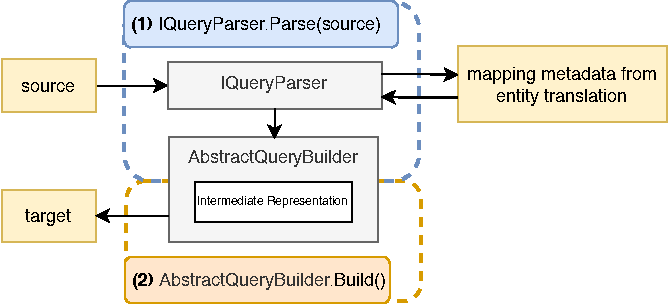
\includegraphics[scale=1]{thesis/img/thesis/04_translate_process_queries.drawio.pdf}
  \caption{Translation process of query with (1) parsing and (2) building phase.}
  \label{fig:translation_process_query}
\end{figure}

The parser must be provided an entire method or a repository class to obtain sufficient context. Queries may lack important context, such as the database table and column names, which are only accessible through entity mapping. While this is not necessary for \acrshort{sql} queries, it is especially important for \acrshort{linq} queries, which abstract away the underlying database structure. Therefore, it is assumed that query translation occurs after entity translation is completed and the mapping is stored in the intermediate representation. This representation can then be passed to the query parser to look up metadata.

\begin{example}
\small
This example demonstrates a simple repository class using \acrshort{efcore} with one method. 
It could serve as an input to the translation tool. A method argument is captured in the query and used as a parameter. 
\begin{lstlisting}[language=CSharp]
class CustomerRepository(DbContext context)
{
    List<Customer> GetCustomersWithLimitOver(int limit)
    {
        return ctx.Customers
            .Where(c => c.CreditLimit > limit)
            .OrderByDescending(c => c.Name)
            .ToList();
    }
}
\end{lstlisting}
\qed
\end{example}

\subsection{Query builder}

Query builder constructs the abstract instructions internally, without exposing them to the parser. The abstract query builder instead exposes a set of methods and builds these instructions internally.

As the parser begins processing a query or any subquery, it calls the method \texttt{Push}. When leaving the nesting, it calls its counterpart \texttt{Pop}. The builder keeps track of the start of the nesting and, when it ends, collects all the instructions, wrapping them in the \texttt{SUBQUERY} instruction. When parsing is complete, the list of instructions should contain a single element. It must be either a \texttt{SUBQUERY} or a \texttt{SET\_OPERATION} instruction.

The \texttt{SetOperation} assumes the parser just left a nested query and \texttt{SUBQUERY} is the last in the list. The builder remembers the set operation and when returning from nesting on the same level, it constructs a \texttt{SET\_OPERATION} instruction, setting both side and the operation type.
Methods such as \texttt{From}, \texttt{Project}, \texttt{Select}, \texttt{Join}, \texttt{OrderBy}, \texttt{GroupBy}, and \texttt{Having} correspond directly to the respective instruction types, including their arguments. 

Listing~\ref{lst:aqb} presents the structure of the \texttt{AbstractQueryBuilder} class. All methods that build the internal instruction representation are public and fully implemented. Two abstract methods are declared and must be implemented by concrete framework implementations. The \texttt{BuildSQL} method serves to generate output queries using raw \acrshort{sql}. For Dapper and PetaPoco, which support only \acrshort{sql} queries, the purpose is straightforward. Other frameworks that primarily use \acrshort{linq} also offer an option to execute raw \acrshort{sql}. In such cases, this method enables that functionality if desired by the user. Otherwise, the \texttt{Build} method is exposed to generate a \acrshort{linq}-based variant. The builder does not declare any private abstract methods. As query structures differ significantly across frameworks, the internal implementation is left entirely to a developer.

 \begin{lstlisting}[caption={AbstractQueryBuilder class structure}, language=pseudo, label={lst:aqb}]
abstract class AbstractQueryBuilder
    
public: 
    Push() {...}
    Pop() {...}
    SetOperation(operationType) {...}
    From(table, alias) {...}
    Project(table, attribute, alias, aggregationFn) {...}
    Select(condition) {...}
    Join(table1, table2, joinType, condition) {...}
    OrderBy(table, attribute, direction) {...}
    GroupBy(table, attribute) {...}
    Having(condition) {...}
    
    abstract Build() : string;
    abstract BuildSQL() : string;
 \end{lstlisting}

 
%LINQ má obecně opačné pořadí instrukcí, ale zároveň že zatímco v SQL je pořadí dané, v LINQu se může měnit a tím se může kompletně změnit semantics
During the generation of each (sub)query, the builder may need to reorder the corresponding instructions. For example, in \acrshort{sql}, projection appears at the beginning of the query but references attributes defined later. Whereas in \acrshort{linq}, it typically comes at the end, just before result materialization. \acrshort{sql} generally follows a fixed linear structure of its query parts. On the other hand, in \acrshort{linq} the order of method calls is not completely fixed, and reordering them can completely alter the semantics of the query.

Algorithm~\ref{alg:query_builder_main} demonstrates how an \acrshort{sql} builder could be implemented. In this case, the builder does not directly generate \acrshort{sql}. The concrete \acrshort{sql} syntax generation is delegated to a visitor pattern. This approach enables swapping out visitor implementations based on a desired \acrshort{sql} dialect.

As previously discussed, the builder assumes the first instruction is either a set operation or a subquery. For a subquery instruction, it directly generates the syntax using the \texttt{BuildSelectQuery} method (see Algorithm \ref{alg:query_builder_buildselect}). In the case of a set operation instruction, it invokes the same method on its two subqueries and concatenates their output with the appropriate set operation. Internally, \texttt{BuildSelectQuery} can also be repeatedly called to generate nested subqueries, for example, within condition trees.

Algorithm~\ref{alg:query_builder_buildselect} illustrates the operation of the \texttt{BuildSelectQuery} method. It delegates its tasks to specialized methods while correctly ordering query parts by invocation order. Each of these methods is responsible for choosing the necessary instructions. Algorithms~\ref{alg:query_builder_buildprojection} and \ref{alg:query_builder_build_selection} demonstrate implementations for \texttt{BuildProjectionPart} and \texttt{BuildSelectionPart} respectively. The remaining methods follow a similar approach and are not explicitly demonstrated.

\texttt{BuildProjectionPart} collects all projection instructions, invoking the visitor to generate syntax. If no projection is declared, the query defaults to returning all available results. \texttt{BuildSelectionPart} gathers all selection instructions. While \acrshort{sql} permits only a single \texttt{WHERE} condition, \acrshort{linq} allows multiple invocations of the \texttt{Where} method, which are semantically connected by a conjunction. This is reflected by merging them into a tree under a conjunction node. The selection instruction already contains condition trees parsed by the query parser. The visitor is called on the final tree, producing the corresponding \acrshort{sql} condition.

One query builder is passed among the functions, sequentially constructing the final query. The main algorithm concludes by encapsulating the generated query within a repository class, considering the specific framework conventions, query source object, and associated methods.

\begin{algorithm}[!htp]
    \footnotesize
    \DontPrintSemicolon

    \SetKw{return}{return}
    
    \KwIn{$inst$ -- abstract instructions built in parsing phase\;}
    \myinput{$visitor$ -- concrete SQL visitor implementation\;}

    $firstInstruction$ = $inst$[0]\;
    $query$ = empty string\;

    \If{\textup{$firstInstruction$ is SubQueryInstruction}} {
        $query$ = BuildSelectQuery($firstInstruction$)\;
    }
    \ElseIf{\textup{$firstInstruction$ is SetOperationInstruction}}{
        $left$ = BuildSelectQuery($firstInstruction$.Left)\;
        $right$ = BuildSelectQuery($firstInstruction$.Right)\;
        $operation$ = $visitor$.Visit($firstInstruction$)\;

        $query$ = $left$ + $operation$ + $right$\;
    }

    $result$ = WrapQueryInRepository($query$)\;

    \return{$result$}
    \caption{\acrshort{sql}  query builder}
    \label{alg:query_builder_main}
\end{algorithm}

\begin{algorithm}[!htp]
    \footnotesize
    \DontPrintSemicolon

    \SetKw{return}{return}
    
    \KwIn{$subq$ -- SubQuery instruction\;}
    \myinput{$sb$ -- string builder\;}

    $inst$ = $subq$.Instructions\;
    \BlankLine
    BuildProjectionPart($sb$, $inst$)\;
    BuildFromPart($sb$, $inst$)\;
    BuildJoinPart($sb$, $inst$)\;
    BuildSelectionPart($sb$, $inst$)\;
    BuildGroupByPart($sb$, $inst$)\;
    BuildHavingPart($sb$, $inst$)\;
    BuildOrderByPart($sb$, $inst$)\;
    \BlankLine
    \return{$sb$.ToString()}
    \caption{\acrshort{sql}  query builder - function \texttt{BuildSelectQuery}}
    \label{alg:query_builder_buildselect}
\end{algorithm}

\begin{algorithm}[!htp]
    \footnotesize
    \DontPrintSemicolon

    \SetKw{return}{return}
    
    \KwIn{$instructions$ -- list of current subquery instructions\;}
    \myinput{$sb$ -- string builder\;}
    \myinput{$visitor$ -- concrete SQL visitor implementation\;}

    $projections$ = $instructions$.OfType(ProjectInstruction)\;

    \If{\textup{$projections$.IsEmpty()}}{
        $sb$.AppendLine(`SELECT *')\;
        \return
    }

    $sb$.Append(`SELECT')\;
    \ForEach{\textup{$proj$ in $projections$}}{
        $sb$.Append($proj$.Accept(visitor))\;
    }
    $sb$.AppendLine()\;
    
    \caption{\acrshort{sql}  query builder - function \texttt{BuildProjectionPart}}
    \label{alg:query_builder_buildprojection}
\end{algorithm}

\begin{algorithm}[!htp]
    \footnotesize
    \DontPrintSemicolon

    \SetKw{return}{return}
    
    \KwIn{$instructions$ -- list of current subquery instructions\;}
    \myinput{$sb$ -- string builder\;}
    \myinput{$visitor$ -- concrete SQL visitor implementation\;}

    $selections$ = $instructions$.OfType(SelectInstruction)\;

    \If{\textup{$projections$.IsEmpty()}}{
        \return
    }

    $sb$.Append(`WHERE')\;
    $andNode$ = new AndOperandNode\;
    \ForEach{\textup{$sel$ in $projections$}}{
        $andNode$.AddChild($sel$.ConditionTree)\;
    }
    $sb$.Append($andNode$.Accept(visitor))\;
    $sb$.AppendLine()\;
    \caption{\acrshort{sql}  query builder - function \texttt{BuildSelectionPart}}
    \label{alg:query_builder_build_selection}
\end{algorithm}

\FloatBarrier\
\subsection{Query parser}

% stejné jako v předchozí kapitole, jen má parser přístup k IR

% pseudocodes of parsing - visitor using Roslyn's CSharpSyntaxWalker over LINQ 

Similarly to the parser for entities and mapping, query parser interface defines only two methods, as demonstrated in Listing~\ref{lst:qparser}. The \texttt{CanParse} method receives a content type and indicates whether the parser is capable of processing it. And the \texttt{Parse} method initiates the actual process. The method has an additional argument to accept entity mapping intermediate representation from which it can obtain necessary metadata.  

 \begin{lstlisting}[caption={IQueryParser interface structure}, language=pseudo, label={lst:qparser}]
interface IQueryParser

public:
    CanParse(contentType) : boolean;
    Parse(source, entityMap);
 \end{lstlisting}

 Algorithm~\ref{alg:query_parser_main} demonstrates how a parser over a \acrshort{linq} query can work. It leverages multiple visitors sharing a common interface, as shown in Listing~\ref{lst:syntaxvisitor}. Each visitor handles specific \acrshort{linq} methods, indicating the compatibility using the \texttt{CanVisit} method. Subsequently, the \texttt{Visit} method extracts relevant information from each \acrshort{linq} method call and forwards it to the query builder.

 Algorithm~\ref{alg:query_parser_main} uses .NET Roslyn compiler, specifically its \texttt{CSharpSyntaxWalker} class\footnote{\url{https://learn.microsoft.com/en-us/dotnet/api/microsoft.codeanalysis.csharp.csharpsyntaxwalker}}. Roslyn was previously used for parsing entity classes in Chapter \ref{chapter:entity_translation}, where the entity parser directly extracted information from the entire syntax tree. \texttt{CSharpSyntaxWalker} enables implementing the visitor pattern, allowing the Roslyn syntax analyzer to invoke appropriate methods upon visiting each syntax node. Algorithm~\ref{alg:query_parser_main} selectively overrides methods to target only relevant expressions. Given that \acrshort{linq} query consists of chained method calls, the \texttt{VisitInvocationExpression} is specifically overridden to handle each method call.

 % example of two visitors
 Algorithm~\ref{alg:query_parser_where} illustrates a visitor for the selection method. In \texttt{CanVisit}, it verifies whether a given node is a member access to a \texttt{Where} method. During parsing, it extracts the lambda expression representing the condition. The lambda body is subsequently parsed by a condition tree parser, and the resulting condition tree is passed to the query builder within the select instruction.
 Algorithm~\ref{alg:query_parser_orderby} handles multiple ordering method calls, namely \texttt{OrderBy}, \texttt{OrderByDescending}, \texttt{ThenBy}, and \texttt{ThenByDescending}. The sort direction is explicitly indicated by the method name. It extracts the entity and property from the lambda expression, typically structured as \texttt{entity => entity.Property}. Here, the parser utilizes the entity mapping information to convert entity and property names to their corresponding table and column names. The remaining visitors employe a similar strategy and are not explicitly shown.

  \begin{lstlisting}[caption={ISyntaxVisitor interface structure}, language=pseudo, label={lst:syntaxvisitor}]
interface ISyntaxVisitor

public:
    CanVisit(expressionSyntax) : boolean;
    void Visit(expressionSyntax, parserContext);
 \end{lstlisting}

 \begin{algorithm}[!htp]
    \footnotesize
    \DontPrintSemicolon

    \SetKwProg{Fn}{override function}{:}{end}
    \SetKwFunction{FVisitInvocationExpression}{VisitInvocationExpression}
    \SetKw{return}{return}
    \SetKw{break}{break}

    \KwIn{$S_{in}$  -- source code of repository class\;}
    \myinput{$builder$  -- instance of \texttt{AbstractQueryBuilder}\;}
    \myinput{$entityMap$  -- entity mapping intermiediate representation\;}
    \myinput{$visitors$  -- list of all implementations of \texttt{ISyntaxVisitor}\;}
    
    $root$ = GetSyntaxTreeRoot($S_{in}$)\;

    $builder.Push()$\;

    \BlankLine
    \tcp{Method inherited from \texttt{CSharpSyntaxWalker}}
    \Fn{\FVisitInvocationExpression{$node$}}{
        $base$.VisitInvocationExpression($node$)\;

        \ForEach{\textup{$visitor$ in $visitors$}}{
            \If{\textup{$visitor$.CanVisit($node$)}}{
                $visitor$.Visit($node$, this)\;
            }
            \break\;
        }
    }
    $builder.Pop()$\;
    
    \caption{\acrshort{linq} query parser}
    \label{alg:query_parser_main}
\end{algorithm}


\begin{algorithm}[!htp]
    \footnotesize
    \DontPrintSemicolon

    \SetKw{return}{return}
    \SetKwProg{Fn}{function}{:}{end}
    \SetKwFunction{FCanVisit}{CanVisit}
    \SetKwFunction{FVisit}{Visit}

    \tcp{Is this LINQ function for selection?}
    \Fn{\FCanVisit{$expressionSyntax$}}{
        $isMemberAccess$ = $expressionSyntax$.Expression is MemberAccessExpressionSyntax\;
        $isWhere$ = $expressionSyntax$.Name.Identifier == `Where'\;

        \return $isMemberAccess$ and $isWhere$\;
    }

    \tcp{Parse filter condition}
    \Fn{\FVisit{$expressionSyntax$, $parserContext$}}{
        $arg$ = $expressionSyntax$.GetArguments()[0]\;

        \If{\textup{$arg$ is not LambdaExpressionSyntax}}{
            \return
        }

        $lambdaBody$ = $arg.Body$\;

        $conditionTree$ = $parserContext$.ConditionTreeParser.Parse($lambdaBody$)\;
        
        $parserContext$.QueryBuilder.Select($conditionTree$)\;
    }
    \caption{\acrshort{linq} query parser - implementation of \texttt{WhereVisitor} extending \texttt{ISyntaxVisitor}}
    \label{alg:query_parser_where}
\end{algorithm}

\begin{algorithm}[!htp]
    \footnotesize
    \DontPrintSemicolon

    \SetKw{return}{return}
    \SetKwProg{Fn}{function}{:}{end}
    \SetKwFunction{FCanVisit}{CanVisit}
    \SetKwFunction{FVisit}{Visit}

    \tcp{Is this LINQ function for ordering?}
    \Fn{\FCanVisit{$expressionSyntax$}}{
        $isMemberAccess$ = $expressionSyntax$.Expression is MemberAccessExpressionSyntax\;
        $isOrderBy$ = $expressionSyntax$.Name.Identifier in (`OrderBy', `OrderByDescending', `ThenBy', `ThenByDescending')\;

        \return $isMemberAccess$ and $isOrderBy$\;
    }

    \tcp{Get ordering target and direction}
    \Fn{\FVisit{$expressionSyntax$, $parserContext$}}{
        $arg$ = $expressionSyntax$.GetArguments()[0]\;

        \If{\textup{$arg$ is not LambdaExpressionSyntax}}{
            \return
        }

        $lambdaBody$ = $arg.Body$\;
        \BlankLine
        $entity$ = getEntityFromExpression($lambdaBody$)\;
        $table$ = $parserContext$.EntityMap.GetTableForEntity($entity$)\;
        \BlankLine
        $property$ = getPropertyFromExpression($lambdaBody$)\;
        $column$ = $parserContext$.EntityMap.GetColumnForProperty($entity$, $property$)\;
        \BlankLine
        $isAsc$ = $expressionSyntax$.Identifier in (`OrderBy', `ThenBy')\;
        \BlankLine
        $parserContext$.QueryBuilder.OrderBy($table$, $column$, $isAsc$)\;
    }
    \caption{\acrshort{linq} query parser - implementation of \texttt{OrderByVisitor} extending \texttt{ISyntaxVisitor}}
    \label{alg:query_parser_orderby}
\end{algorithm}
    


%\subsection{Translation process}

\FloatBarrier
\begin{example}
\small

The established abstraction and algorithms enable the demonstration of the complete translation process. Figure~\ref{fig:translation_complete_query} visualizes the conversion of an \acrshort{efcore} \texttt{linq} query into Dapper using \acrshort{sql}. The example query consists of two filter conditions followed by result sorting. For clarity, only the method containing the query is displayed. 

The translation begins with the parser analyzing the query and converting each component into an intermediate representation. In this example, the query translates into three instructions. To construct the \texttt{FROM} instruction, the parser consults the entity mapping to associate the entity with a corresponding database table. The entity mapping is repeatedly accessed multiple times to map  properties within each method call.

The two \texttt{Where} method calls are converted into a single \texttt{WHERE} instruction with a condition tree. This structure allows for accurately representing complex conditions as nested trees, maintaining the correct order of operation hierarchy. Finally, the \texttt{Order} method call is converted into an appropriate ordering instruction.

In the subsequent phase, the builder translates these intermediate instructions into an \acrshort{sql} query. Since the original query does not specify projections explicitly, it defaults to selecting all available columns. Each instruction is converted into its respective \acrshort{sql} syntax, with multiple conditions merged into a single conjunction. Ultimately, the query is encapsulated into a method, taking into account that Dapper operates directly over a database connection rather than a \texttt{DbContext}. This method would be wrapped in a repository class, receiving the connection object as a constructor parameter, likely using dependency injection. 
\qed
\end{example}

\begin{figure}[!htp]
  \centering
  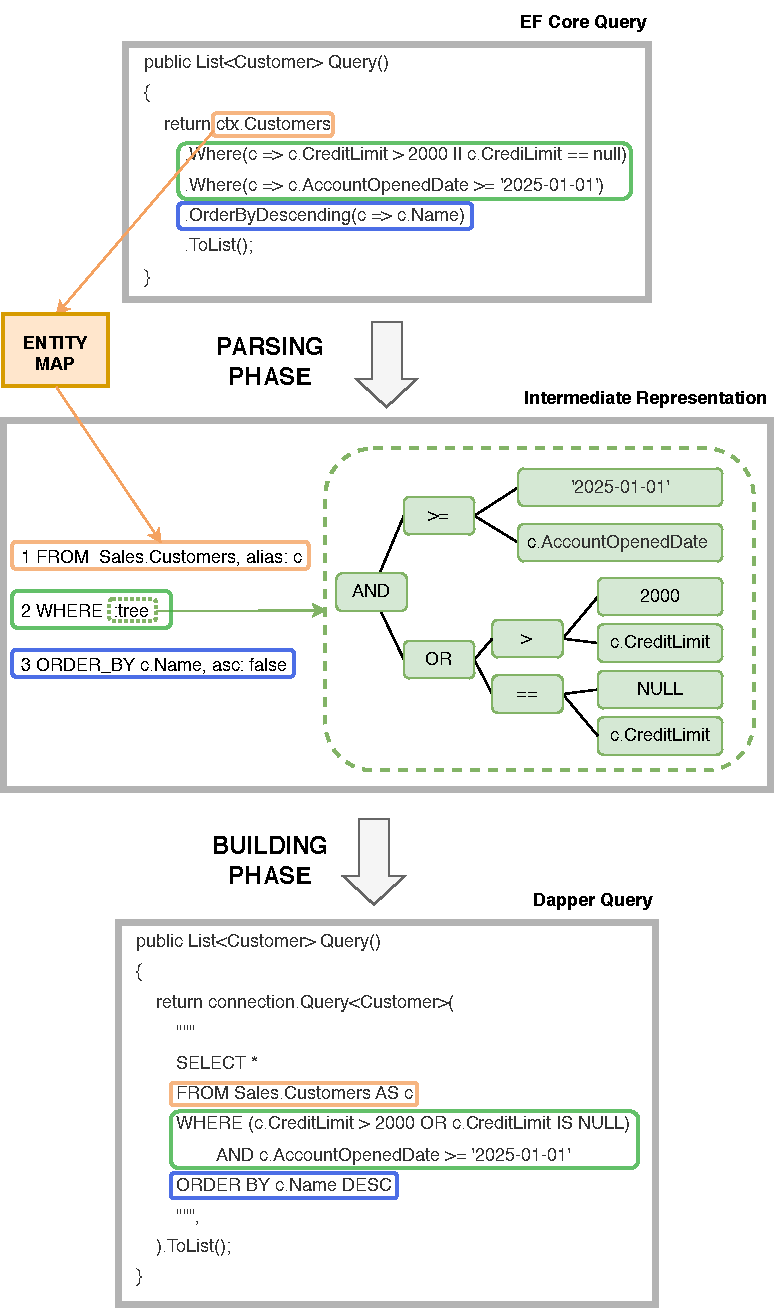
\includegraphics[scale=1]{thesis/img/thesis/04_parsing_building_queries.drawio.pdf}
  \caption{Translation of \acrshort{efcore} LINQ query to SQL in Dapper.}
  \label{fig:translation_complete_query}
\end{figure}